\begin{figure}
    \begin{minipage}[c]{0.4\textwidth}
        \caption{We use the product of many Gaussian-initialized matrices as our \textit{"correlated-initialized"} weight matrix. To show the levels of correlation versus the number of matrices in the product, we plot the averaged cosine similarities of weight vectors. Notice that the number of nodes $N$ in hidden layers are all 6.}
        \label{fig:sec3_sim1}
    \end{minipage}\hfill
    \begin{minipage}[c]{0.5\textwidth}
        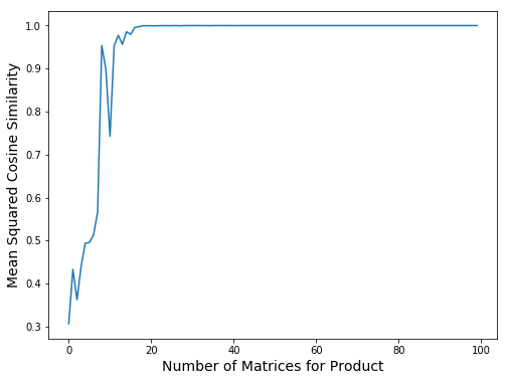
\includegraphics[width=\textwidth]{CorrelatedInitialization}
    \end{minipage}
\end{figure}